\documentclass[tikz,border=10pt]{standalone}
% Shared UMM figure style (journal-consistent palette + line weights)
\usepackage{tikz}
\usepackage{pgfplots}
\pgfplotsset{compat=1.18}
\usetikzlibrary{arrows.meta,calc,positioning,decorations.pathmorphing,patterns,shapes.geometric,fit,backgrounds}
% Palette: grayscale + single accent (deep teal)
\definecolor{ummAccent}{HTML}{0B6E6E}
\definecolor{ummAccentLight}{HTML}{4A9B9B}
\definecolor{ummDark}{HTML}{1A1A1A}
\definecolor{ummGray}{HTML}{555555}
\definecolor{ummLightGray}{HTML}{AAAAAA}
\definecolor{ummFill}{HTML}{E8F2F2}
\definecolor{ummGas}{HTML}{C45C26}
\definecolor{ummGasLight}{HTML}{F0C4A8}
\definecolor{ummGalaxy}{HTML}{2C3E50}
\definecolor{ummLens}{HTML}{0B6E6E}
\pgfplotsset{
  umm axis/.style={
    axis lines=left,
    axis line style={ummDark, line width=0.8pt},
    tick style={ummDark, line width=0.6pt},
    tick label style={font=\footnotesize, ummDark},
    label style={font=\small, ummDark},
    title style={font=\small\bfseries, ummDark},
    grid=both,
    major grid style={ummLightGray, opacity=0.35, line width=0.3pt},
    minor grid style={ummLightGray, opacity=0.15, line width=0.2pt},
    every axis plot/.append style={line width=1.3pt},
    legend style={font=\footnotesize, draw=ummLightGray, fill=white, fill opacity=0.92, text opacity=1},
    clip=false,
  },
}
\newcommand{\ummLineW}{1.25pt}
\newcommand{\ummLineWthin}{0.9pt}
\tikzset{
  umm arr/.style={-{Latex[length=2.2mm,width=1.6mm]}},
}

\begin{document}
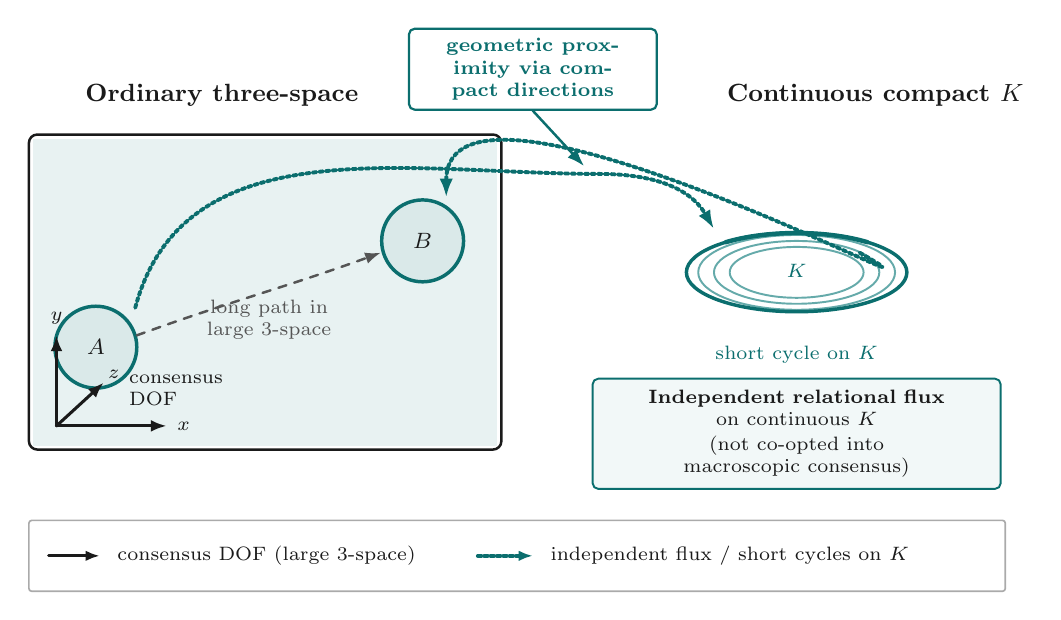
\begin{tikzpicture}[font=\small, line cap=round, line join=round]
  % Outer reserved frame (ensures all content sits inside tight bbox with padding)
  % Content span: x in [0, 12.6], y in [-1.15, 5.35]

  % --- Left: ordinary 3-space with two distant points ---
  \node[font=\bfseries\small, ummDark] at (2.6, 5.25) {Ordinary three-space};
  \draw[ummDark, line width=0.9pt, rounded corners=3pt]
    (0.15,0.75) rectangle (6.15,4.75);
  \fill[ummFill] (0.2,0.8) rectangle (6.1,4.7);

  % Two distant regions A and B
  \fill[ummAccent!15] (1.0,2.05) circle (0.52);
  \draw[ummAccent, line width=\ummLineW] (1.0,2.05) circle (0.52);
  \node[font=\footnotesize\bfseries, ummDark] at (1.0,2.05) {$A$};

  \fill[ummAccent!15] (5.15,3.4) circle (0.52);
  \draw[ummAccent, line width=\ummLineW] (5.15,3.4) circle (0.52);
  \node[font=\footnotesize\bfseries, ummDark] at (5.15,3.4) {$B$};

  % Long path in 3-space (dashed gray)
  \draw[ummGray, dashed, line width=\ummLineWthin,
        -{Latex[length=2mm,width=1.5mm]}]
    (1.52,2.2) to[out=20,in=200] (4.62,3.25);
  \node[font=\scriptsize, ummGray, align=center] at (3.2,2.4)
    {long path in\\large 3-space};

  % Consensus axes
  \draw[ummDark, line width=1.1pt, -{Latex[length=2mm]}] (0.5,1.05) -- (1.9,1.05)
    node[right, font=\scriptsize] {$x$};
  \draw[ummDark, line width=1.1pt, -{Latex[length=2mm]}] (0.5,1.05) -- (0.5,2.2)
    node[above, font=\scriptsize] {$y$};
  \draw[ummDark, line width=1.1pt, -{Latex[length=2mm]}] (0.5,1.05) -- (1.1,1.6)
    node[above right, font=\scriptsize, inner sep=1pt] {$z$};
  \node[font=\scriptsize, ummDark, align=left, anchor=west] at (1.3,1.5)
    {consensus\\DOF};

  % --- Right: continuous compact K ---
  \node[font=\bfseries\small, ummDark] at (10.9, 5.25) {Continuous compact $K$};
  \begin{scope}[shift={(9.9,3.0)}]
    \foreach \s in {1.25, 1.05, 0.85} {
      \draw[ummAccentLight, line width=0.7pt, opacity=0.85]
        (0,0) ellipse ({\s} and {\s*0.38});
    }
    \draw[ummAccent, line width=\ummLineW] (0,0) ellipse (1.4 and 0.5);
    \draw[ummAccent, line width=1.6pt]
      (50:1.4 and 0.5) arc[start angle=50, end angle=130, x radius=1.4, y radius=0.5];
    \node[font=\scriptsize\bfseries, ummAccent] at (0,0.02) {$K$};
  \end{scope}
  \node[font=\scriptsize, ummAccent, align=center] at (9.9,1.95)
    {short cycle on $K$};

  % Geometric proximity via K
  \draw[ummAccent, line width=1.4pt, densely dotted,
        -{Latex[length=2.4mm,width=1.7mm]}]
    (1.5,2.55) to[out=75,in=180] (7.4,4.25)
    to[out=0,in=120] (8.85,3.55);
  \draw[ummAccent, line width=1.4pt, densely dotted,
        -{Latex[length=2.4mm,width=1.7mm]}]
    (10.7,3.25) to[out=-30,in=90] (5.45,3.95);

  % Callout in open whitespace between column titles (not over diagram lines);
  % near-opaque pale fill so text stays fully legible; arrow to proximity path.
  % Sit above the path in the central gap; titles sit farther left/right so no overlap.
  \node[font=\scriptsize\bfseries, ummAccent, align=center,
        draw=ummAccent, line width=0.8pt, rounded corners=2pt,
        fill=white, fill opacity=0.97, text opacity=1,
        inner sep=3.5pt, text width=2.9cm]
    (proxylab) at (6.55,5.58)
    {geometric proximity via compact directions};
  \draw[ummAccent, line width=0.9pt, -{Latex[length=2.2mm,width=1.6mm]}]
    (proxylab.south) -- (7.2,4.35);

  % Independent flux label: fully inside frame (text width constrained)
  \node[font=\scriptsize, ummDark, align=center, text width=4.9cm,
        draw=ummAccent, line width=0.7pt, rounded corners=2pt,
        fill=ummFill, fill opacity=0.55, text opacity=1,
        inner sep=4pt]
    at (9.9,0.95)
    {\textbf{Independent relational flux}\\
     on continuous $K$\\[0.15em]
     {\scriptsize (not co-opted into macroscopic consensus)}};

  % Legend strip (fully inside bbox)
  \draw[ummLightGray, line width=0.6pt, rounded corners=1pt]
    (0.15,-1.05) rectangle (12.55,-0.15);
  \fill[white, opacity=0.92] (0.18,-1.02) rectangle (12.52,-0.18);
  \draw[ummDark, line width=1.1pt, -{Latex[length=1.8mm]}] (0.4,-0.6) -- (1.05,-0.6);
  \node[font=\scriptsize, anchor=west, ummDark] at (1.15,-0.6)
    {consensus DOF (large 3-space)};
  \draw[ummAccent, line width=1.3pt, densely dotted, -{Latex[length=1.8mm]}]
    (5.85,-0.6) -- (6.55,-0.6);
  \node[font=\scriptsize, anchor=west, ummDark] at (6.65,-0.6)
    {independent flux / short cycles on $K$};
\end{tikzpicture}
\end{document}
